% !TeX spellcheck = en_GB
\section{Numerics}
\subsection{High Performance Computations}
It is important to make the program as fast as possible.
Indeed, the faster the program goes, the more data it will generate (within the same amount of time).
This data will be used for numerical analysis and we will also use it for interpretation.
Therefore, with more data, we have more knowledge, and we can make smarter guesses.

There are two main ways to make a program faster:
use a better algorithm, or 
use a faster implementation.
For example, in the test of primality of a number $n$, we may test factors only up to $\sqrt{n}$, instead of up to $n$.
A better implementation simply means optimisation inside the computer (i.e. on operations that are made, types that are used...).
We will try to optimise both.


\subsubsection{Algorithm Optimisation}
\label{algorithmOptimisation}
We can optimize an algorithm by optimizing (decreasing) the number of operations, or by using mathematical scheme (usually cancellations).

\paragraph{Optimize instructions}
Optimizing instructions usually comes through optimizing loops (stopping loops as soon as possible, avoiding extra loops...).
For example, the following two algorithms create the same list of coefficients for the $q$-series of $\Delta$.

\textbf{\textit{Algorithm 1:}}
\begin{algorithmic}
	\color{CodeColor}
	\Require $L \geq 1$
	\State{$f \leftarrow zeros(L)$}\Comment{Empty list of length $L$}
	\State{n=0}
	\While{$n < L$}
		\If{$(\sqrt{n}-1) \% 2 = 0$}
			\State{$f[n]=1$}
		\EndIf
	\EndWhile
\end{algorithmic}

\textit{\textbf{Algorithm 2:}}
\begin{algorithmic}
	\color{CodeColor}
	\Require $L \geq 1$
	\State{$f \leftarrow zeros(L)$}\Comment{Empty list of length $L$}
	\State{$id=1$}
	\State{$i=1$}
	\While{$id < L$}
		\State{$f[id] = 1$}
		\State{$i += 2$}
		\State{$id = i^2$}
	\EndWhile
\end{algorithmic}

However, the second algorithm is significantly more efficient: the loop is faster as it only goes through odd squares instead of all numbers, and it has no condition to check.
An efficient algorithm may be \textit{harder} to understand, but is actually \textit{better} (in terms of performance).

\paragraph{Mathematical ruse}
As we are working modulo 2, there are obviously many cancellations, which will make the calculations \textit{faster}.
It is an opportunity we shouldn't miss to make the algorithms \textit{stronger}.
% harder, better, faster, stronger



\subsubsection{Implementation Approach}
As explained above, investigations on which tool will be the more suitable for the computation is an important part.
Of course, the best would be to find a programming language that can already deal with modular forms modulo two.
Unfortunately, this (yet) doesn't exist.
There are packages that have modular forms implemented, but none with modular forms modulo two specifically.
The goal of looking at modulo two is to conclude more than what we know in general.
So using what has already been done in general to make computations modulo two won't be useful.

We realize that there is no other way than just creating a package for modular forms modulo two on our own.
In fact, this is what we will do later, but before, we want to determine the tools to build this package.
Modular forms modulo 2 come from maths, so it makes sense to use a \href{https://en.wikipedia.org/wiki/High-level_programming_language}{high level programming language}.
For scientific computing nowadays, there are two main \href{https://en.wikipedia.org/wiki/Open-source_model}{open source} languages: \href{https://en.wikipedia.org/wiki/Python_(programming_language)}{Python} and \href{https://en.wikipedia.org/wiki/Julia_(programming_language)}{Julia}.
Each having various packages to work with.

We will test a selection of major ones.



\subsubsection{Choice of Implementation}
Now it is time to wonder how to represent modular forms modulo 2.
We have seen above that a modular form modulo 2 in fact have two representations: one as an infinite $q$-series, and one as a finite $\Delta$-polynomial.
As we want (later on) to compute Hecke operators of these forms, we will need, at some point to use the $q$-series representation.
In fact, this will be one of the crucial points, since it is an infinite series.
The way we represent infinite objects in computers, which have only a finite amount of components (memory addresses, say), is to only store informations up to a cutting point.
This is equivalent (somewhat) to the asymptotic notation in mathematics.
In the case of $q$-series of modular forms, we will store only the few first hundred/thousand/million coefficients.

This means that we will represent a modular form via its $q$-series, witch will be stored as a list.
We investigate the best ways (time wise) to do basic operations to decide what technology to use.
The operations tested are creating the $q$-series of $\Delta$, and squaring it (both storing coefficients up to some power \texttt{LENGTH}, the length of the list used).

There are various techniques to store lists in a computer, the main ones being continuous lists, linked lists, and sparse lists.
Continuous and linked lists are both dense lists.

\paragraph{Dense Technique}
Dense storage means that we store each values of the list (next to each other, or with a link to the next).
No element of the list is skipped.
There are various ways to implement this technique:
\subparagraph{Pure Python}
Using the Python language, this is the most elementary way to go.
It represents all the $q$-coefficients with the default linked list python object.
(code in appendix \ref{code:PurePython}).
\subparagraph{NumPy Python}
\href{https://fr.wikipedia.org/wiki/NumPy}{NumPy} is the most well known scientific computing library for Python.
It interfaces with C objects to provide very fast features (such as lists).
(code in appendix \ref{code:NumPyPython}).
\subparagraph{Dense Julia}
Julia is well-known as both high level and very fast language.
Julia naturally supports lists, that we can use to represent modular forms.
(code in appendix \ref{code:DenseJulia}).

\paragraph{Sparse Technique}
As all coefficients of the $q$-series are just $0$ or $1$, and that most of the time, they are $0$, we can represent a modular forms by storing only the coefficients for which it is non-zero.
This method (storing only non-zero values) is known as \href{https://en.wikipedia.org/wiki/Sparse_matrix}{sparse representation}.
We can implement this technique in both Python and Julia:
\subparagraph{Sparse Python}
We can adapt the previous code to use Python's linked lists as index of a sparse list.
Note that in general, we would need a second list to store values, but there are only $0$s and $1$s, we can take as convention that all stored indices have value $1$ and all non-store have value $0$.
(code in appendix \ref{code:SparsePython}). 
\subparagraph{Sparse Julia}
Julia has a very convenient built-in sparse module.
This is particularly interesting, since the built-in type already have nice methods.
(code in appendix \ref{code:SparseJulia}).

\paragraph{Speed Comparison}
We can now compare the speed of each implementation to compute $q$-series.
If we do that for various number of coefficients, we may obtain a graph of the following type (it is sightly dependent on the machine that execute the code, but the shape remains).

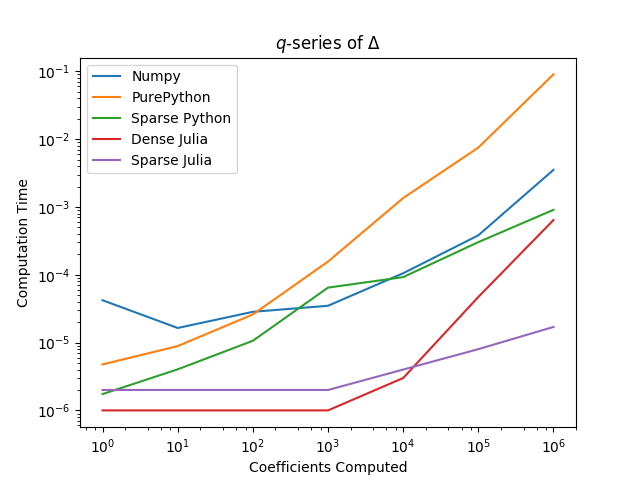
\includegraphics{speed_comparison_delta}

For small computations, the implementation doesn't make a big difference.
However, for large computations, it seems that the sparse methods do better.
It makes sense, since sparse representations are typically used for objects with more than 95\% of zeros, which is the case for modular forms modulo 2.

For a more precise analysis, we now compare the speed of each implementation to compute $q$-series of $\Delta$ and $\Delta^2$
\footnote{$\Delta^2$ itself isn't part of our space $\mathcal{F}$, but it will be useful as we will compute $\Delta^{2k+1} = \Delta^{2k-1}\cdot \Delta^2$. So it makes sense to be concerned about it.}.
The following table is obtained for $10^6$ coefficients computed (i.e. up to $q^{10^6}$).
Note that $\mathcal{O}(q^{10^6})$ will be standard for the rest of this paper.

\begin{center}
	\begin{tabular}{r||l|l}
		 & $\Delta$ & $\Delta^2$\\
		\hline\hline
		Pure Python   & 0.08263147 & 0.26249526 \\
		NumPy Python  & 0.00138761 & 0.16163688 \\
		Dense Julia   & 0.000648   & 0.001698   \\
		Sparse Python & 0.00095099 & 0.00134479 \\
		Sparse Julia  & 0.000021   & 0.000034   \\
	\end{tabular}
\end{center}

From this table, it is clear that the fastest implementation is the one using sparse lists (so called "sparse vectors") in Julia.
Therefore, we will use this technique.
It is nice to remark that the Pure Python implementation was 7720 times slower than the Sparse Julia one.
We see here the importance of choosing the right tool to implement an algorithm.

This ratio would even be greater considering the bad algorithm presented before \ref{algorithmOptimisation}.



\subsection{Creating the library}
It is clear now that the code should be done with Julia and it's Sparse objects.
Now, as all the library should be created from the beginning, it is a good idea to pack all of it in a Julia module.
Doing so, no code will be repeated for each small task.



\subsubsection[Main Module]{ModularFormsModuloTwo.jl}
The code will be divided in a many files, for convenience.

\paragraph{Code Architecture}
The main function are direct parts of the module, and the pre-calculated data part is written in a sub-folder, detailed next paragraph.
Here is a visualization of the organisation (the "architecture"):

% code architecture draw
\tikzset{
	file/.style={
		rectangle,
		rounded corners,
		draw=black, very thick,
		minimum height=4.2cm,
		minimum width=3.8cm,
		inner sep=2pt,
		text width=3.7cm,
	},
}
\tikzset{
	submodule/.style={
		rectangle,
		rounded corners,
		draw=black, thin,
		minimum height=1.5cm,
		minimum width=4.6cm,
		inner sep=2pt,
		text width=4.7cm,
	},
}
\begin{tikzpicture}
%% nodes
\coordinate(top) at (0,0);
\node[file, text width=6.25cm] (MFmod2) at (top){
	\begin{tabular}{l}
	\textbf{ModularFormsModuloTwo.jl}\\
	$\cdot$ ModularForm (\textit{type})\\
	$\cdot$ ModularFormList (\textit{type})\\
	$\cdot$ \textit{Printing functions}\\
	\\
	\\
	\\
	\end{tabular}
};
\node[file, below of = top, node distance=5cm] (gene){
	\begin{tabular}{l}
	\textbf{generator.jl}\\
	$\cdot$ zero ($0$)\\
	$\cdot$ one ($1$)\\
	$\cdot$ delta ($\Delta$)\\
	$\cdot$ delta\_k ($\Delta^k$)\\
	\\
	\\
	\end{tabular}
};
\node[file, left of = gene, node distance=4cm] (arithm){
	\begin{tabular}{l}
	\textbf{arithmetic.jl}\\
	$\cdot$ addition ($+$)\\
	$\cdot$ multiplication ($*$)\\
	$\cdot$ square (²)\\
	$\cdot$ power (${}^{\boxed{}}$)\\
	\textbf{equality.jl}\\
	$\cdot$ eq ($\overset{?}{=}$)\\
	\end{tabular}
};
\node[file, right of = gene ,node distance=4cm] (reco){
	\begin{tabular}{l}
	\textbf{recognizer.jl}\\
	$\cdot$ to\_q ($\Delta \to q$)\\
	$\cdot$ to\_$\Delta$ ($q \to \Delta$)\\
	$\cdot$ drop\_error ($q \circlearrowleft$)\\
	\\
	\\
	\\
	\end{tabular}
};
\node[file, right of = reco, node distance=4.5cm] (Hecke){
	\begin{tabular}{l}
	\textbf{HeckeOperator.jl}\\
	$\cdot$ Hecke ($T_p$)\\
	\\
	\\
	\\
	\\
	\end{tabular}
};
\node[submodule, right of = MFmod2, node distance=7cm, thin] (Data){
	\begin{tabular}{l}
	\textbf{Data (submodule)}\\
	\textit{(load precalculated data)}\\
	\end{tabular}
};
%% links
\path (MFmod2) edge (arithm);
\path (MFmod2) edge (gene);
\path (MFmod2) edge (reco);
%\path (MFmod2) edge (Hecke);
\path (MFmod2) edge (+6,-2);
\path (+6,-2) edge (Hecke);
\path (MFmod2) edge (Data);
\end{tikzpicture}
\begin{center}
	Major functions of the module and their repartitions into file (represented by boxes).
\end{center}



\paragraph{Files Details}
We will detail here the important and interesting parts of the code.
For more details, the reader may refer to the source code, witch is commented and documented.
\subparagraph{Basics Operations}
Basic operations on modular forms modulo 2 are defined in \texttt{arithmetic.jl} (see \ref{code:arithmetic} or \url{https://github.com/pauldubois98/ModularFormsModuloTwo.jl/blob/master/src/arithmetic.jl}).
All of these algorithms have been optimised as much as possible (i.e. cutting loops as soon as possible, and iterate through "ones" only, as most coefficients are zero).
\subparagraph{Equality up to known}
It might be useful to compare two modular form up to some coefficients (perhaps if $f_1$ is known up to $q^n$ and $f_2$ up to $q^m$, we can compare them up to $q^{\min{n,m}}$).
This equality test is defined in \texttt{equality.jl} (see \ref{code:equality} or \url{https://github.com/pauldubois98/ModularFormsModuloTwo.jl/blob/master/src/equality.jl}).
\subparagraph{Generators of $\mathcal{F}$}
As modular forms modulo 2 are polynomials of $\Delta$, we need to ba able to generate the $q$-series of powers of $\Delta$.
Such functions are defined in \texttt{generator.jl} \footnote{\texttt{generators.jl} generates $\Delta$ and then uses the power function from \texttt{arithmetic.jl}.} (see \ref{code:generators} or \url{https://github.com/pauldubois98/ModularFormsModuloTwo.jl/blob/master/src/generators.jl}).
Here, the optimization is not trivial:
To calculate $\Delta^{31}$ (say), the most trivial way is to do $\Delta \cdot \Delta \cdots \Delta$ with 30 multiplications.
But what is done in fact inside the library is much faster: we calculate $\Delta$, $\Delta^2 = \Delta \cdot \Delta$, $\Delta^4 = \Delta^2 \cdot \Delta^2$, ... until $\Delta^{16}$, and then $\Delta^{31} = \Delta^{16} \cdot \Delta^8 \cdot \Delta^4 \cdot \Delta^2 \cdot \Delta$.
Doing like this, only 8 multiplications were needed (against 30 with the naïve method).
On may think that 3 was an example particularly good for this technique, but if we take another example, say 32, we would turn 31 multiplication to 5.
In fact, in general, to calculate $\Delta^n$ this second method need a maximum of $\log_2(n)^2$ multiplications against $n-1$ for the first one.
So it really is a much faster algorithm.\footnote{In fact, half of the operations are squaring modular forms, which is much faster than a usual multiplication. This this algorithm is even better than stated.}
\subparagraph{Hecke Operators}
The only formula we have to calculate Hecke operators, is using the $q$-representation of modular forms.
Therefore, the Hecke operators are taking a modular forms under $q$-representation as input (together with a prime $p$).
Note that when applying a Hecke operator, we loose a lot of informations on it's expansion:
If $f$ is known up to $q^n$, then $T_p|f$ will only be known up to $q^{n/p}$.
This means that we should be careful when applying Hecke operator.

Hecke operators are implemented in the file \texttt{HeckeOperator.jl} (see \ref{code:HeckeOperator} or \url{https://github.com/pauldubois98/ModularFormsModuloTwo.jl/blob/master/src/HeckeOperator.jl})
\subparagraph{Recognise the trick?}
\label{recogniseTrick}
This part of the module us probably the most important, and it is the one that differ the most form any other computing technique.

We start by noting that it is easy to go from the $\Delta$ representation of a modular form to the $q$ representation: it suffices to choose an arbitrary $n$, and calculate all coefficients up to $q^n$, using the series expansion of $\Delta$.
This step is necessary to calculate Hecke operators.

Now, one may ask if it is possible to go back from the $q$-representation to the $\Delta$-representation of a modular form.
In general, this is not possible.
\textbf{But}
If we have some assumptions on the modular form, then it may become possible.
For example, if we know that the maximum degree (in terms of $\Delta$) of $f$ is n, and that we know it's $q$-coefficients up to n:
then $f$ may be written as $f = \sum_{k \leq n} \mu_k \Delta^k$, so the set $\{ \Delta^k | k \leq n \}$ acts as a basis, and it is just a matter of finding the matching coefficients $\mu_k$.
This is in fact possible, and that is how the function \texttt{to\_delta()} is made possible.

Now, once we have the $\Delta$ representation of a modular form, we potentially have as many $q$-coefficients as we want.
This may seem weird or even magical, since we assumed only finitely many $q$-coefficients were known.
In fact, we can use this fact to drop the numerical error that calculating a Hecke operator may have produced.

Such kind of calculations are rather unusual in computer science: usually computers approximates objects, and this approximation error is never given back.
But with modular forms modulo two, we can take back the approximation error.

This method will now be referred as exact computations. [may I create this name?]

It is implemented in the file \texttt{recognizer.jl} (see \ref{code:recognizer} or \url{https://github.com/pauldubois98/ModularFormsModuloTwo.jl/blob/master/src/recognizer.jl}).
\subparagraph{Global}
The last file, \texttt{ModularFormsModuloTwo.jl} is the one that creates the link between all the small part of programs written in other files.
It also defines a few general objects, such as types and printing functions.
For more details, see (\ref{code:ModularFormsModuloTwo} or \url{https://github.com/pauldubois98/ModularFormsModuloTwo.jl/blob/master/src/ModularFormsModuloTwo.jl})
\subsubsection[Sub Module]{(Pre-calculated) Data}
Data is natively part of the ModularFormModuloTwo.jl module, but it is treated internally as a sub-component, for better organisation.



\paragraph{Code Architecture}
This time, the architecture is much easier:

\tikzset{
	subfile/.style={
		rectangle,
		rounded corners,
		draw=black, very thick,
		minimum height=1.2cm,
		minimum width=5.2cm,
		inner sep=2pt,
		text width=5.5cm,
		align=center,
	},
}
\begin{tikzpicture}
%% nodes
\coordinate(top) at (0,0);
\node[submodule, align=center] (data) at (top){
	\textbf{\LARGE Data}
};
\node[subfile, below of = top, node distance=3cm] (storage){
	storage.jl
};
\node[subfile, right of = storage, node distance=6cm] (delta){
	delta\_file\_maker.jl
};
\node[subfile, right of = delta ,node distance=6cm] (primes){
	Hecke\_primes\_file\_maker.jl
};
\node[subfile, above of = primes, node distance=3cm] (powers){
	Hecke\_powers\_file\_maker.jl
};
%% links
\path (data) edge (storage);
\path (data) edge (delta);
\path (data) edge (primes);
\path (data) edge (powers);
\end{tikzpicture}

\paragraph{Files Details}
We will detail here an overview of what each file achieve.
For more details, the reader may look at the source code, which is highly commented, and quite explicit in general.
\begin{itemize}
	\item \texttt{storage.jl} (see \ref{code:storage} or \url{https://github.com/pauldubois98/ModularFormsModuloTwo.jl/blob/master/src/data/storage.jl}): This is the only file to be called outside of the Data sub-module.
	\item \texttt{delta\_file\_maker.jl} (see \ref{code:deltaFileMaker} or \url{https://github.com/pauldubois98/ModularFormsModuloTwo.jl/blob/master/src/data/delta_file_maker.jl}): The program in this file generates the $q$-coefficients lists for a range of powers of $\Delta$.
	\item \texttt{Hecke\_primes\_file\_maker.jl} (see \ref{code:HeckePrimesFileMaker} or \url{https://github.com/pauldubois98/ModularFormsModuloTwo.jl/blob/master/src/data/Hecke_primes_file_maker.jl}): The program in this file calculates the $\Delta$-representation lists for a range of Hecke operators $T_p$ and range of powers of $\Delta$.
	\item \texttt{Hecke\_powers\_file\_maker.jl} (see \ref{code:HeckePowersFileMaker} or \url{https://github.com/pauldubois98/ModularFormsModuloTwo.jl/blob/master/src/data/Hecke_powers_file_maker.jl}): The program in this file calculates the $\Delta$-representation lists for a range of powers of Hecke operators $T_3$ and $T_5$ and range of powers of $\Delta$.
\end{itemize}



\subsubsection{Open-Source}
This library is completely open-source.
Anyone is welcome to contribute.
Anyone can use it (for free).

\subsubsection{Official}
This module is now registered as an official Julia package.
To use all the code form this library, a new user will just need to type:
\begin{minted}{julia}
julia> using Pkg
julia> Pkg.add(PackageSpec(url="https://github.com/pauldubois98/ModularFormsModuloTwo.jl"))
\end{minted}
It is convenient that all the algorithms developed in this module can be used just by importing the package, which can be done in a minute.

\subsubsection{Online Documentation}
As it usually comes wit open-sources packages, ModularFormsModuloTwo.jl has an \href{https://pauldubois98.github.io/ModularFormsModuloTwo.jl/}{online documentation} (see \url{https://pauldubois98.github.io/ModularFormsModuloTwo.jl/}).




\subsection{Finding Coefficients $a_{ij}(p)$}
\label{finding_a_ij(p)}
\subsubsection{Strategy}
We want to find the coefficients $a_{ij}$ such that 
\begin{equation}
\label{eq:coefficientsEquate}
	T_p = \sum_{i+j \geq 1} a_{ij}(p)T_3^iT_5^j \tag{$*$}
\end{equation}
(with $a_{ij}(p) \in \mathbb{F}_2$).
Note that this is a finite sum, since Hecke operators are nilpotent.

The strategy is as follows: we use the module we developed.
It allows us to compute the (exact) $\Delta$-representation of $T_p|\Delta^k$ and $\sum_{i+j \geq 1} a_{ij}(p) T_3^iT_5^j|\Delta^k$ for many $k$, $p$, $i$ and $j$.
Now, since \eqref{eq:coefficientsEquate} should hold for all modular forms $f \in \mathcal{F}$, it has to holds, in particular, for all $\Delta^k$ (with $k$ and odd integer).
Thus, we will plug successive $\Delta^k$ and equate coefficients.
This will eventually give all $a_ij(p)$.

\subsubsection{Algorithm}
As explained before, we plot $\Delta^k$ successively for a range of $k$.
In reality, most of the terms of the sum in \ref{eq:coefficientsEquate} are zeros.
This is both nice and not good:
It is nice because it makes the system is easy to solve.
But it also makes all coefficients in front of zeros terms being undetermined.
This implies that we need to plug larger powers of $\Delta$ to fix coefficients.
And bigger powers of $\Delta$ ask for heavier computations (and now we see how important it was to optimize the modular forms modulo 2 module).

As this algorithm is the heart of all computations, we give a pseudo-code simplified version:
\begin{algorithmic}
	\color{CodeColor}
	\Require $MAX_K$ \Comment{Maximum power $\Delta^k$ for which $T_p|\Delta^k$ and $T_3^iT_5^j|\Delta^k$ are known (computed)}
	\Require $MAX_I$ \Comment{Minimum $i \in \N$ such that $T_3^i|\Delta^{MAX_K} \neq 0$}
	\Require $MAX_J$ \Comment{Minimum $j \in \N$ such that $T_5^j|\Delta^{MAX_K} \neq 0$}
	\ForAll{$p \in \primes$, $p>2$}
		\Comment{We compute the map $a_{ij}(p)$ for each specific odd $p$ prime}
		\State{$a_p$ is a $MAX_I \times MAX_J$ 2-dimensional matrix} \Comment{$a_p[i,j]$ will correspond to $a_{ij}(p)$}
		\State{Fill $a_p$ for known values (i.e. for $i+j \leq 2$}
		\For{$k < MAX_K$}
			\State{$f = T_p|\Delta^k$}
			\State{$LIST_a$} \Comment{The list of $a_p[i,j]$ to fix using $\Delta^k$ iteration}
			\State{$LIST_f$} \Comment{The corresponding list of modular forms $T_3^iT_5^j|\Delta^k$}
			\For{$0 \leq i \leq MAX_I$}
				\For{$0 \leq j \leq MAX_J$}
					\If{$a_p[i,j]=1$}
						\State{$f += T_3^iT_5^j|\Delta^k$} \Comment{Add $1 * T_3^iT_5^j|\Delta^k$ to $f$}
					\ElsIf{$a_p[i,j]=0$}
						\State{Pass} \Comment{Add $0 * T_3^iT_5^j|\Delta^k$ to $f$}
					\Else \Comment{$a_p[i,j]$ is unset in this case.}
						\State{Append $a_p[i,j]$ to $LIST_a$} \Comment{We add $a_p[i,j]$ to the list}
						\State{Append $T_3^iT_5^j|\Delta^k$ to $LIST_f$} \Comment{We add $T_3^iT_5^j|\Delta^k$ to the list}
					\EndIf
				\EndFor
			\EndFor
			\State{Find $a_p[i,j]$ in $LIST_a$ that solve that system $f = \sum a_p[i,j] T_3^iT_5^j|\Delta^k$} \Comment{using built-in linear solver, for efficiency}
		\EndFor
		\State{Output $a_p$}
	\EndFor
\end{algorithmic}
The implementation of this algorithm (in Julia) is in \ref{code:a_ij(p)calculation}.



\subsubsection{Computations Limitations}
Here, we discuss the bounds to put in the algorithm, for a decent amount of data, and a descent amount of computation time.

\paragraph{Computing Hecke of Large Primes Versus Large Powers}
Here, we compare the difficulty to compute Hecke operators for large primes ($T_p$ for $p >> 2$), against the difficulty to compute Hecke operators for large powers of Hecke operators ($T_3^iT_5^j$ for $i,j >> 1$).

\subparagraph{Computing Hecke Operators for Large Primes}
When calculating a Hecke operator $T_p$ for a modular form $f$, the maximum known coefficient is $q^{\frac{N}{p}}$ if $f$ is known for coefficients up to $q^{N}$.
This means that we can compute the $\Delta$ representation for $T_p|f$ only if we know it will have a degree (in terms of $\Delta$) of maximum $\frac{N}{p}$.
Thus, if we choose to compute $a_{ij}(p)$ for $p \leq P$, it means that $\degree{T_p|f} \leq \frac{N}{P} = K$.

\subparagraph{Computing Hecke Operators for Large Powers}
Now, at a first thought, $T_p$ isn't too pathological compared to $T_3^iT_5^j$ for large $i$ and $j$, since the maximum known coefficient would be $q^{\frac{N}{3^i5^j}}$ if $f$ is known for coefficients up to $q^{N}$.

But in fact, we can apply a trick here:
Once we know $T_3|f$ (once we computed it's $q$-representation), we straight calculate the $\Delta$-representation, and then get back to the $q$-representation with no "lose of coefficients".
This may look weird at first, since we have the $q$-representation of $T_3|f$, and we need it to calculate $T_3^2|f$.
However, we known the $q$-representation of $T_3|f$ with some coefficients lost.
And the fact that we go back to the $\Delta$-representation allows us to drop the numerical error.
Doing this again and again, there is no lose at all in the coefficients calculated.

This is why exact computations (this is the name we gave to this trick) is crucial for this algorithm.
In fact, for powers of Hecke operators, we only need to compute the $q$-representations of modular forms up to $5 \ \degree{f}$, since each $T_3$ or $T_5$ will lose at most $\nicefrac{4}{5}$ of the $q$-coefficients.

\subparagraph{Conclusion}
Thus, the part which use to be the most pathological in fact becomes much nicer than the other: Calculating Hecke operators for large powers is easier than for large primes.

\paragraph{Reasonable Bounds}
Here, we give limits used in the actual computations.

It seems that using $q$ series capped at $q^{10^6}$ is reasonable (i.e. computations will be a few days long).
We would like to compute $a_ij(p)$ for small $i,j$ and $p \leq 10^4$.

So the setup (in the same notation as above) is $N=10^6$, $P=10^4$, so $K=10^2$.
Then the algorithm will compute as much $a_{ij}(p)$ as possible, for each $p \leq P$.
This maximum can in fact be calculated implicitly:
$a_{ij}(p)$ will be computed if and only if $T_3^iT_5^j|f$ is non-zero for one of the forms $f$ plugged.
As we plug powers of $\Delta$ up to $K$, this means $a_{ij}(p)$ will be computed for all $p \leq P$ if and only if $k \leq K$, where $k$ is the odd integer with code $[i,j]$.

\subsubsection{Results}
Here, we will give results for the prime $p=19$.
There are many links in this section, if the reader in interested in all the data calculated (it won't fit in this paper).

\paragraph{Expansions of $T_p$}
We have the following extension:
$$
T_{19} = T_3^1T_5^0 + T_3^3T_5^0 + T_3^1T_5^4 + T_3^3T_5^2 + T_3^1T_5^6 + T_3^5T_5^2 + T_3^3T_5^6 + T_3^7T_5^2 + T_3^9T_5^0 + \dots
% + T_3^1T_5^{10} + T_3^7T_5^4 + T_3^9T_5^2 + T_3^{11}T_5^0
% + T_3^1T_5^{12} + T_3^5T_5^8 + T_3^{11}T_5^2 + T_3^{13}T_5^0 + T_3^3T_5^{12} + T_3^7T_5^8 + T_3^9T_5^6 + T_3^{11}T_5^4 + T_3^{13}T_5^2 + T_3^3T_5^{14} + T_3^7T_5^{10} + T_3^{11}T_5^6 + T_3^{15}T_5^2 + T_3^{17}T_5^0
$$
Writing $x = T_3$ and $y = T_5$, this is:
$$
T_{19} = x^1y^0 + x^3y^0 + x^1y^4 + x^3y^2 + x^1y^6 + x^5y^2 + x^3y^6 + x^7y^2 + x^9y^0 + x^1y^{10} + x^7y^4 + x^9y^2 + x^{11}y^0 + \dots
% + x^1y^{12} + x^5y^8 + x^{11}y^2 + x^{13}y^0 + x^3y^{12} + x^7y^8 + x^9y^6 + x^{11}y^4 + x^{13}y^2 + x^3y^{14} + x^7y^{10} + x^{11}y^6 + x^{15}y^2 + x^{17}y^0
$$
For expansions of other primes, please visit \href{https://pauldubois98.github.io/HeckeOperatorsModuloTwo/T_p_extensions/}{this web site}:\\ \url{https://pauldubois98.github.io/HeckeOperatorsModuloTwo/T_p_extensions/}.

For $p=19$, we can also look at $a_{ij}(p)$ as an infinite 2-dimensional table:
\begin{center}
	\begin{tabular}{|c||c|c|c|c|c|c|c|c|c|c|c|c|c|c|c|c|}
		\hline
		\textbf{$ T_19$} & \textbf{$ T_5^{0} $} & \textbf{$ T_5^{1} $} & \textbf{$ T_5^{2} $} & \textbf{$ T_5^{3} $} & \textbf{$ T_5^{4} $} & \textbf{$ T_5^{5} $} & \textbf{$ T_5^{6} $} & \textbf{$ T_5^{7} $} & \textbf{$ T_5^{8} $} & \textbf{$ T_5^{9} $} & \textbf{$ T_5^{10} $} & \textbf{$ T_5^{11} $} & \textbf{$ T_5^{12} $} & \textbf{$ T_5^{13} $} & \textbf{$ T_5^{14} $} & \textbf{$ T_5^{15} $} \\
		\hline
		$ T_3^{0} $ & 0 & 0 & 0 & 0 & 0 & 0 & 0 & 0 & 0 & 0 & 0 & 0 & 0 & 0 & 0 & 0 \\
		$ T_3^{1} $ & 1 & 0 & 0 & 0 & 1 & 0 & 1 & 0 & 0 & 0 & 1 & 0 & 1 & 0 & 0 & 0 \\
		$ T_3^{2} $ & 0 & 0 & 0 & 0 & 0 & 0 & 0 & 0 & 0 & 0 & 0 & 0 & 0 & 0 & 0 & 0 \\
		$ T_3^{3} $ & 1 & 0 & 1 & 0 & 0 & 0 & 1 & 0 & 0 & 0 & 0 & 0 & 1 & 0 & 1 & 0 \\
		$ T_3^{4} $ & 0 & 0 & 0 & 0 & 0 & 0 & 0 & 0 & 0 & 0 & 0 & 0 & 0 & 0 & 0 &  \\
		$ T_3^{5} $ & 0 & 0 & 1 & 0 & 0 & 0 & 0 & 0 & 1 & 0 & 0 & 0 & 0 & 0 &  &  \\
		$ T_3^{6} $ & 0 & 0 & 0 & 0 & 0 & 0 & 0 & 0 & 0 & 0 & 0 & 0 & 0 &  &  &  \\
		$ T_3^{7} $ & 0 & 0 & 1 & 0 & 1 & 0 & 0 & 0 & 1 & 0 & 1 & 0 &  &  &  &  \\
		$ T_3^{8} $ & 0 & 0 & 0 & 0 & 0 & 0 & 0 & 0 & 0 & 0 & 0 &  &  &  &  &  \\
		$ T_3^{9} $ & 1 & 0 & 1 & 0 & 0 & 0 & 1 & 0 & 0 & 0 &  &  &  &  &  &  \\
		$ T_3^{10} $ & 0 & 0 & 0 & 0 & 0 & 0 & 0 & 0 & 0 &  &  &  &  &  &  &  \\
		$ T_3^{11} $ & 1 & 0 & 1 & 0 & 1 & 0 & 1 & 0 &  &  &  &  &  &  &  &  \\
		$ T_3^{12} $ & 0 & 0 & 0 & 0 & 0 & 0 & 0 &  &  &  &  &  &  &  &  &  \\
		$ T_3^{13} $ & 1 & 0 & 1 & 0 & 0 & 0 &  &  &  &  &  &  &  &  &  &  \\
		$ T_3^{14} $ & 0 & 0 & 0 & 0 & 0 &  &  &  &  &  &  &  &  &  &  &  \\
		$ T_3^{15} $ & 0 & 0 & 1 & 0 &  &  &  &  &  &  &  &  &  &  &  &  \\
		$ T_3^{16} $ & 0 & 0 & 0 &  &  &  &  &  &  &  &  &  &  &  &  &  \\
		$ T_3^{17} $ & 1 & 0 &  &  &  &  &  &  &  &  &  &  &  &  &  &  \\
		$ T_3^{18} $ & 0 &  &  &  &  &  &  &  &  &  &  &  &  &  &  &  \\
		\hline
	\end{tabular}

	Here, blanks are coefficients not computed.
\end{center}
For tables of other primes, please visit \href{https://pauldubois98.github.io/HeckeOperatorsModuloTwo/a_ij_p/}{this web site}:\\ \url{https://pauldubois98.github.io/HeckeOperatorsModuloTwo/a_ij_p/}.

Now, we will later be interested in the map $p \to a_{ij}(p)$, so it makes sense for each pair $(i,j)$, to list the \textit{1-primes} (i.e. the set $\{ p \in \primes \mid a_{ij}(p) = 1 \}$) or the 0-primes 
This is what we do in the following table:
\begin{center}
	\begin{tabular}{|r|l|}
		\hline
		\textbf{$a_{ij}$} & \textbf{$ \lbrace p \in \primes \mid a_{ij}(p) = 1 \rbrace $} \\
		\hline
		$ a_{0 1} $ & 5, 13, 29, 37, 53, 61, 101, 109, 149, 157, 173, 181, 197, 229, 269, 277, 293, 317, 349, ...\\
		$ a_{1 0} $ & 3, 11, 19, 43, 59, 67, 83, 107, 131, 139, 163, 179, 211, 227, 251, 283, 307, 331, 347, ...\\    
		$ a_{0 2} $ & 17, 41, 97, 137, 193, 241, 313, 401, 409, 433, 449, 457, 521, 569, 641, 673, 761, 769, ...\\
		$ a_{1 1} $ & 7, 23, 31, 47, 71, 79, 103, 127, 151, 167, 191, 199, 223, 239, 263, 271, 311, 359, 367, ...\\
		$ a_{2 0} $ & 17, 73, 89, 97, 193, 233, 241, 281, 401, 433, 449, 601, 617, 641, 673, 769, 929, 937, ...\\
		$ a_{0 3} $ & 13, 29, 37, 101, 149, 173, 181, 317, 349, 389, 557, 661, 677, 709, 733, 757, 773, 997, ...\\
		$ a_{1 2} $ & 11, 59, 67, 83, 107, 131, 179, 211, 251, 331, 347, 379, 419, 499, 523, 547, 587, 619, ...\\
		$ a_{2 1} $ & 13, 37, 53, 61, 101, 157, 173, 277, 373, 389, 509, 541, 557, 677, 701, 709, 773, 797, ...\\
		$ a_{3 0} $ & 11, 19, 67, 107, 131, 283, 307, 331, 419, 443, 467, 523, 547, 563, 571, 587, 619, 643, ...\\
		$ a_{0 4} $ & 73, 89, 113, 233, 353, 577, 593, 601, 937, 1153, 1201, 1289, 1433, 1601, 1609, 1721, ...\\
		$ a_{1 3} $ & 23, 31, 71, 79, 103, 127, 151, 191, 223, 239, 263, 359, 431, 463, 479, 503, 631, 647, ...\\
		$ a_{2 2} $ & 17, 41, 73, 89, 113, 233, 241, 257, 313, 353, 401, 409, 433, 457, 601, 761, 809, 937, ...\\
		$ a_{3 1} $ & 7, 79, 167, 199, 239, 311, 383, 431, 439, 463, 487, 599, 607, 719, 727, 743, 751, 823, ...\\
		$ a_{4 0} $ & 41, 113, 257, 313, 337, 409, 457, 577, 761, 809, 881, 1129, 1249, 1553, 1657, 1889, ...\\
		$ a_{0 5} $ & 13, 53, 61, 101, 109, 157, 173, 197, 269, 317, 349, 389, 421, 461, 613, 653, 661, 701, ...\\
		$ a_{1 4} $ & 11, 19, 67, 107, 131, 163, 179, 211, 227, 251, 283, 307, 331, 347, 419, 491, 643, 811, ...\\
		$ a_{2 3} $ & 29, 37, 53, 61, 101, 149, 157, 173, 197, 269, 293, 389, 397, 421, 541, 557, 613, 653, ...\\       
		$ a_{3 2} $ & 11, 19, 43, 83, 107, 131, 163, 211, 251, 347, 379, 419, 443, 467, 491, 523, 563, 571, ...\\
		$ a_{4 1} $ & 13, 53, 101, 149, 157, 173, 181, 229, 317, 373, 397, 421, 461, 613, 661, 701, 709, ...\\
		$ a_{5 0} $ & 11, 43, 59, 67, 83, 139, 163, 251, 283, 419, 467, 499, 547, 587, 619, 643, 659, 811, ...\\
		$ \dots $ & \\
		\hline
	\end{tabular}

	Table of 1-primes
\end{center}
Again, for complete tables, please visit \href{https://pauldubois98.github.io/HeckeOperatorsModuloTwo/a_ij_p/a_ij_p-1.html}{this web site}:\\ \url{https://pauldubois98.github.io/HeckeOperatorsModuloTwo/a_ij_p/a_ij_p-1.html}.

Note that tables for \textit{0-primes} (i.e. the set $\{ p \in \primes \mid a_{ij}(p) = 0 \}$) may be found \href{https://pauldubois98.github.io/HeckeOperatorsModuloTwo/a_ij_p/a_ij_p-0.html}{here}:\\
\url{https://pauldubois98.github.io/HeckeOperatorsModuloTwo/a_ij_p/a_ij_p-0.html}.




\subsection{Finding Governing Fields}
\subsubsection{Strategy}
As it is usually the case with computations, this algorithm will not give a proof that the considered field is a governing field.
What we will do, is to check that for sufficiently many primes, the field we consider is a governing field.

\paragraph{Outline of the Algorithm}
Consider the field $L$ extending $\Q$, suppose we suspect it to be a governing field for $a_{ij}$.
We want to check that there exists a subset $S \subseteq G = \Gal{L/\Q}$ that is stable under conjugacy, such that $\Frob{L/\Q}{p} \in S$ if and only if $a_{ij}(p)=1$.
That is $\Frob{L/\Q}{p} \in S$ if $a_{ij}(p)=1$ and $\Frob{L/\Q}{p} \not \in S$ if $a_{ij}(p)=0$.

\paragraph{Algorithm}
\label{algo:governingFieldsChecks}
Here is a pseudo-code version of the algorithm used:
\begin{algorithmic}
	\color{CodeColor}
	\State{$MAX_P \in \N$}
	\State{$i,j \in \N$ given}
	\State{$L$ a given  number field, suspected to be a governing field for $a_{ij}$.}
	\State{$G = \Gal{L/\Q}$}
	\State{$Primes-1$ an empty set.}
	\For{$p \in \primes, p<MAX_P, a_{ij}(p)=1$}
		\If{$\Frob{L/\Q}{p} \in Primes-0$}
			\State{Add $\Frob{L/\Q}{p}$ to the set $Primes-1$}
		\EndIf
	\EndFor
	\For{$p \in \primes, p<MAX_P, a_{ij}(p)=0$}
		\If{$\exists F_q \in Primes-0 \text{ s.t. } \Frob{L/\Q}{p} \sim F_q$}
			\State{REJECT!}
		\EndIf
	\EndFor
	\Comment{Accept as not rejected yet.}
	\State{$L$ is a Governing field for $a_{ij}$.}
\end{algorithmic}
The implementation of this algorithm (in Python) is in \ref{code:governingFieldsChecks}.
Note that the hardest part to program is in fact the transition between computer's representation of mathematical objects, and the human readable versions. This part isn't mathematically interesting, so has been hidden in this paper. The interested reader may find complete programs on GitHub (see \url{https://github.com/pauldubois98/HeckeOperatorsModuloTwo/tree/master/GoverningFields}).

\paragraph{Implementation Strategy}
For algebraic computations (such as computing Frobenius elements), many libraries already exist.
However, many (such as SageMath) are limited in terms of degree of field extensions.
This is why we will use a very powerful and respected library: PARI GP.
PARI GP may be used through C, but for simplicity, we will use the the GP language that PARI GP developers suggest.

It isn't easy to connect the Julia computations for the maps $a_{ij}$ and the PARI GP language.
So we will export results from both sides in text files, and analyse it with Python.
Note here that the analysis is just checking if whether or not, the field is a governing field.
All the "difficult" computations are made in very efficient languages (Julia and the highly optimized PARI GP library).
So it is fine, for convenience, to use a slower language as Python for the last step, which isn't computationally fast.



\subsubsection{Frobenian Map Test}


\paragraph{Checking Known Governing Fields}
[It is always good to check, to make the theory stronger (this is usually true in Science, a little bit less in math)]
This will test the algorithms that we use: if the output agrees with the theory, then it is less likely to contain errors.
[results: Serre is right]

\paragraph{Finding Possible New Governing Fields}
[NEW RESULTS!!!]
[results: a04, a03, a30, a40]
[more results? (a05, a50, ...)? => if time]


\nicefrac{}{}
\paragraph{Probabilistic Analysis}
Here, we look for the probability that the results found appeared randomly.
We assume that the Frobenius element of a prime is random for each prime.
then the proba [bla].
[this part is written, but only in my head, at the moment.]



